\documentclass{article}
\usepackage{titling}
\usepackage[utf8]{inputenc}
\usepackage{hyperref}
\usepackage[letterpaper, portrait, margin=1in]{geometry}
\usepackage{enumitem}
\usepackage{threeparttable}
\usepackage{amsmath}
\usepackage{booktabs}
\usepackage{graphicx}
\usepackage{authblk}

\usepackage{hyperref}
\hypersetup{
colorlinks=true,
    linkcolor=black,
    filecolor=black,      
    urlcolor=blue,
    citecolor=black,
}
\usepackage{natbib}

\usepackage{titlesec}

\title{Homework 3 Solutions}
\author{Kelly Lifchez}
\date{\today}
  
\begin{document}
  
\maketitle


\section{Python}

\subsection*{(a) Show that $ln(y_i) = \alpha + ln(\delta)d_i + \gamma\ln(z_i) + \eta_i$}

\begin{align}
        y_i &= e^{\alpha} \delta^{d_i} z_i^{\gamma}  e^{\eta_i} \\
        ln(y_i) &= ln\left( e^{\alpha} \delta^{d_i} z_i^{\gamma}  e^{\eta_i} \right) \\
        ln(y_i) & = ln\left( e^{\alpha} \right) + ln\left( \delta^{d_i} \right) + ln\left( z_i^\gamma \right) + ln\left( e^{\gamma_i} \right) \\
        ln(y_i) & = \alpha ln(e) + ln(\delta)d_i + \gamma ln(z_i) + \eta_i ln(e) \\
        ln(y_i) & = \alpha + ln(\delta) d_i + \gamma ln(z_i) + \eta_i.
    \end{align}

\subsection*{(b) What is the intuitive interpretation of $\delta$?}

$\delta$ can be thought of as the direct effect of treatment, or the treatment effect on the treated group. In other words, $\delta$ represents a scaling or multiplier effect of the treatment on $y_i$. This is because when $d_i = 0$, $\delta$ drops out of the regression equation, and when $d_i = 1$, $\delta$ is included. Specifically: \\

\texttt{When $d_i = 0$, $y_i = e^{\alpha} z_i^{\gamma} e^{\eta_i}$ or $ \ln(y_i) = \alpha + \gamma \ln(z_i) + \eta_i$.} \\

\texttt{And when $d_i = 1$, $y_i = e^{\alpha} \delta^{1} z_i^{\gamma}  e^{\eta_i}$ or $ln(y_i) = \alpha + ln(\delta) (1) + \gamma ln(z_i) + \eta_i$.} \\


That means that in this case, $\delta$ is the direct multiplicative change in kWh due to retrofitting, and $ln(\delta)$ represents the percent change in kWh of electricity used in homes that receive the retrofitting treatment. 

\subsection*{(c) Show that $\frac{\Delta y_i}{\Delta d_i} = \frac{(\delta - 1)}{\delta^{d_i}} y_i$. What is the intuitive interpretation of $\frac{\Delta y_i}{\Delta d_i}$ ?}

\begin{align}
\Delta y_i = y_i (d_i = 1) - yi (d_i = 0)
\end{align}

We know the potential outcomes model: 

\[
y_i = \begin{cases} 
      e^{\alpha} z_i^{\gamma} e^{\eta_i} & \text{if } d_i = 0 \\
      e^{\alpha} \delta z_i^{\gamma}  e^{\eta_i} & \text{if } d_i = 1 
   \end{cases}
\]

Therefore we know that 

\begin{align}
\Delta y_i = (e^{\alpha} \delta z_i^{\gamma}  e^{\eta_i}) - (e^{\alpha} z_i^{\gamma} e^{\eta_i})
\end{align}

Pull out $e^{\alpha} z_i^{\gamma} e^{\eta}$ and get: \\

\begin{align}
\Delta y_i = (\delta - 1) (e^{\alpha} z_i^{\gamma} e^{\eta_i})
\end{align}

Next, find the change in $d_i$: \\

\begin{align}
    \Delta d_i = 1 - 0
\end{align}

So we can then calculate the change in $y_i$ over the change in $d_i$: \\

\begin{align}
    \frac{\Delta y_i}{\Delta d_i} = \frac{(\delta - 1) (e^{\alpha} z_i^{\gamma} e^{\eta_i})}{1 - 0}
    & = (\delta - 1) (e^{\alpha} z_i^{\gamma} e^{\eta_i})
\end{align}

\subsection*{(d) Show that $\frac{\partial y_i}{\partial z_i} = \gamma \frac{y_i}{z_i}$. What is the intuitive interpretation of $\frac{\partial y_i}{\partial z_i}$ when $z_i$ is the size of the home in square feet?}

Star with: 

\begin{align}
    ln(y_i) = \alpha + ln(\delta) (1) + \gamma ln(z_i) + \eta_i
\end{align}

Exponentiate both sides: 

\begin{align}
    y_i = exp(\alpha + ln(\delta) (1) + \gamma ln(z_i) + \eta_i) 
\end{align}

Use the chain rule to take the partial derivative of $y_i$ with respect to $z_i$: 

\begin{align}
    \frac{\partial y_i}{\partial z_i} = (\frac{d}{dz})(exp(\alpha + ln(\delta) (1) + \gamma ln(z_i) + \eta_i)) \\
    & = (\frac{\alpha}{z_i})(y_i) \\
    & = \alpha \frac{y_i}{z_i}
\end{align}

In other words, a 100\% change in $z$ creates a $100 \times \alpha$ percent change in $y$. This can also be thought of as a 1\% change in home square footage leading to an $\alpha$ percent change in kWh of electricity use.  


\newpage
\subsection*{(e) Table of coefficient estimates and marginal effects}

Table \ref{tab:py_ests} shows OLS coefficient estimates and the average marginal effects of each of the variables in the regression model on kWh of electricity. Coefficient estimates provide insight into the direct relationship between an explanatory variable and the outcome variable, while the average marginal effects describe the overall impact of an explanatory variable on an outcome in the context of the entire model.\\
Confidence intervals represent the range in which an estimated parameter will fall 95\% of the time if repeatedly sampled. Confidence intervals in Table \ref{tab:py_ests} are constructed using bootstrapping with 1,000 replications. 

\begin{table}[ht]
\centering
\caption{Coefficient estimates and average marginal effects}
\begin{threeparttable}
\begin{tabular}{lll}
\toprule
 & Coefficients & Marginal effects (dy/dx) \\
\midrule
Retrofit & -0.100000 & -113.980000 \\
  & (-0.11, -0.09) & (-0.79, -0.61) \\
Log(Sqft) & 0.890000 & 0.630000 \\
  & (0.88, 0.91) & (0.0, 0.0) \\
Log(Temp) & 0.280000 & 4.000000 \\
  & (0.04, 0.53) & (0.0, 0.05) \\
Constant & -0.770000 &   \\
  & (-1.88, 0.33) &   \\
Observations & 1000.000000 & 1000.000000 \\
\bottomrule
\end{tabular}

\end{threeparttable}  
\label{tab:py_ests}
\end{table}

\newpage
\subsection*{(f) Graph of average marginal effects}

\begin{figure}[!ht]
    \centering
    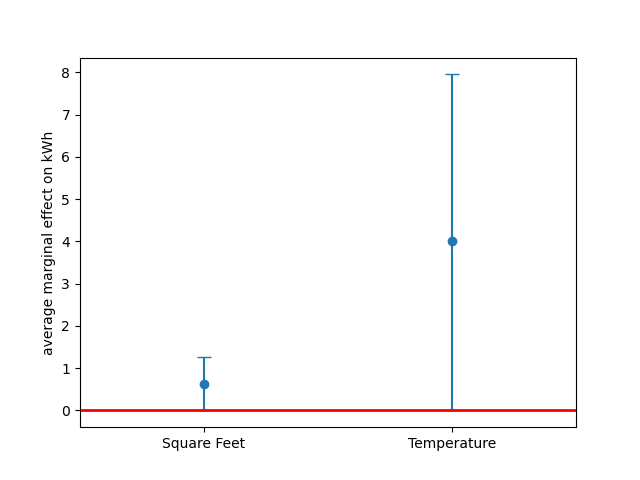
\includegraphics[scale = 0.7]{ame_plot.png}
    \caption{Average marginal effects of home square footage and outdoor temperature}
    \vspace{0.3cm}
    \begin{minipage}{0.78\textwidth}
        \footnotesize Note: The figure depicts the average marginal effects of square footage in a home and outdoor temperature on kWh. Bar caps represent 95\% confidence intervals bootstrapped with 1,000 replications.
    \end{minipage}
    \label{fig:ame_plot}
\end{figure}

% \bibliography{sampleref}
% \bibliographystyle{chicago}

\end{document}
